\documentclass[conference]{IEEEtran}
\IEEEoverridecommandlockouts
% The preceding line is only needed to identify funding in the first footnote. If that is unneeded, please comment it out.
\usepackage{cite}
\usepackage{amsmath,amssymb,amsfonts}
% \usepackage{algorithmic}
\usepackage{graphicx}
\usepackage{textcomp}
\usepackage{xcolor}

% bahasa asing
\usepackage[russian, bahasa]{babel}
\usepackage{CJKutf8}

% Untuk nampilin kode
\usepackage[utf8]{inputenc}
 
\usepackage{listings}
\usepackage{xcolor}
 
\definecolor{codegreen}{rgb}{0,0.6,0}
\definecolor{codegray}{rgb}{0.5,0.5,0.5}
\definecolor{codepurple}{rgb}{0.58,0,0.82}
\definecolor{backcolour}{rgb}{0.95,0.95,0.92}
 
\lstdefinestyle{mystyle}{
    backgroundcolor=\color{backcolour},   
    commentstyle=\color{codegreen},
    keywordstyle=\color{magenta},
    numberstyle=\tiny\color{codegray},
    stringstyle=\color{codepurple},
    basicstyle=\ttfamily\footnotesize,
    breakatwhitespace=false,         
    breaklines=true,                 
    captionpos=b,                    
    keepspaces=true,                 
    numbers=left,                    
    numbersep=5pt,                  
    showspaces=false,                
    showstringspaces=false,
    showtabs=false,                  
    tabsize=2
}
 
\lstset{style=mystyle}

\def\BibTeX{{\rm B\kern-.05em{\sc i\kern-.025em b}\kern-.08em
    T\kern-.1667em\lower.7ex\hbox{E}\kern-.125emX}}
\begin{document}

\title{Perkembangan Teknik Pembelajaran \textit{Artificial Neural Network} hingga \textit{Transformer} dalam Representasi Kata Lintas Bahasa\\}
\author{\IEEEauthorblockN{Ilham Firdausi Putra}
\IEEEauthorblockA{\textit{Sekolah Teknik Elektro dan Informatika} \\
\textit{Institut Teknologi Bandung}\\
Bandung, Indonesia \\
ilhamfputra31@gmail.com}
}

\maketitle

\begin{abstract}
Representasi kata adalah hal yang sangat penting dalam bidang pemrosesan bahasa. Dalam tugas ini, dieksplorasi perkembangan teknik pembelajaran \textit{Artificial Neural Network} hingga \textit{Transformer} dalam representasi teks lintas bahasa. Tidak hanya itu, juga akan dilihat penggunaanya pada perkembangan representasi teks lintas bahasa dari \textit{monolingual mapping} hingga \textit{joint optimization}.
\end{abstract}

\begin{IEEEkeywords}
artificial neural network, transformer, representasi teks lintas bahasa
\end{IEEEkeywords}

\section{Pendahuluan}
Sebagian besar algoritma pembelajaran mesin memerlukan representasi teks dalam bentuk numerik. Untuk hal itu, berkembanglah berbagai teknik untuk merepresentasikan teks sebaik mungkin. Bentuk paling sederhananya adalah pendekatan \textit{one-hot-vector} yang merepresentasikan teks berdasarkan ada atau tidaknya saja. Representasi seperti ini memiliki kekurangan seperti tidak diperhatikannya letak kata dan membesarnya representasi kata seiring membesarnya kosa kata. 

Kekurangan dari representasi \textit{one-hot-ector} dapat diselesaikan dengan \textit{word embedding} seperti Word2vec \cite{b1} yang mempelajari representasi kata sebagai vektor bernilai riil. Pembangunan \textit{word embedding} seperti Word2vec memanfaatkan \textit{Artificial Neural Network} dengan teknik seperti \textit{Continuous Bag of Words} (CBOW) dan Skip-gram.

Representasi teks dengan \textit{word embedding} masih memiliki kelemahan berupa masih dangkalnya representasi. Representasi \textit{word embedding} tidak dapat menangkap interaksi antar kata di kalimat yang kompleks. Oleh karena itu, berkembanglah \textit{language model} seperti XLM \cite{b2} yang tidak hanya belajar di level kata, tetapi sampai dapat memperhatikan konteks di mana kata tersebut berada. Pembangunan \textit{language model} seperti XLM memanfaatkan arsitektur \textit{transformer} yang lebih anyar.
 
Dalam tugas ini akan kita eksplorasi perkembangan penggunaan \textit{Artificial Neural Network} dalam pembangunan \textit{word embedding} lintas bahasa pada Word2vec. Setelah itu kita lihat juga hubungannya ke perkembangan arsitektur \textit{transformer} dalam pembangunan \textit{language model} lintas bahasa seperti XLM. Kita juga akan lihat bagaimana perkembangan representasi lintas bahasa berkembang dari \textit{mapping} secara linear di Word2vec, hingga penggunaan \textit{sub-word} di XLM.

\section{Artificial Neural Network}
Teknik pembelajaran \textit{Artificial Neural Network} (ANN), yang termasuk jenis \textbf{\textit{discriminative}}, pertama kali dimodelkan pada tahun 1943 oleh Warren McCulloch dan Walter Pits \cite{b3}. Pemodelan ini terinspirasi dari cara neuron bekerja di otak. Semenjak itu, berkembang bebagai kemajuan dalam metode dan teknik melakukan pembelajaran dengan ANN. Keefektifan ANN dibuktikan dengan performanya yang berhasil mengalahkan teknik non-ANN di berbagai bidang \cite{b4} \cite{b5}.
	\subsection{Teknik Pembelajaran}
	Sebuah ANN terdiri dari lapisan masukkan (\textit{input}), lapisan tersembunyi (\textit{hidden}), dan lapisan keluaran (\textit{output}) seperti dapat dilihat pada Gambar \ref{fig:ilustrasi_ann}. Tiap garis yang menghubungkan neuron memiliki bobot yang dapat diperbaharui. Dalam pembelajaran, ANN akan melewati fase yang disebut dengan \textit{forward propagation}, \textit{backpropagation}, dan pembaharuan bobot.

	\begin{figure}[htbp]
	    \centerline{
	    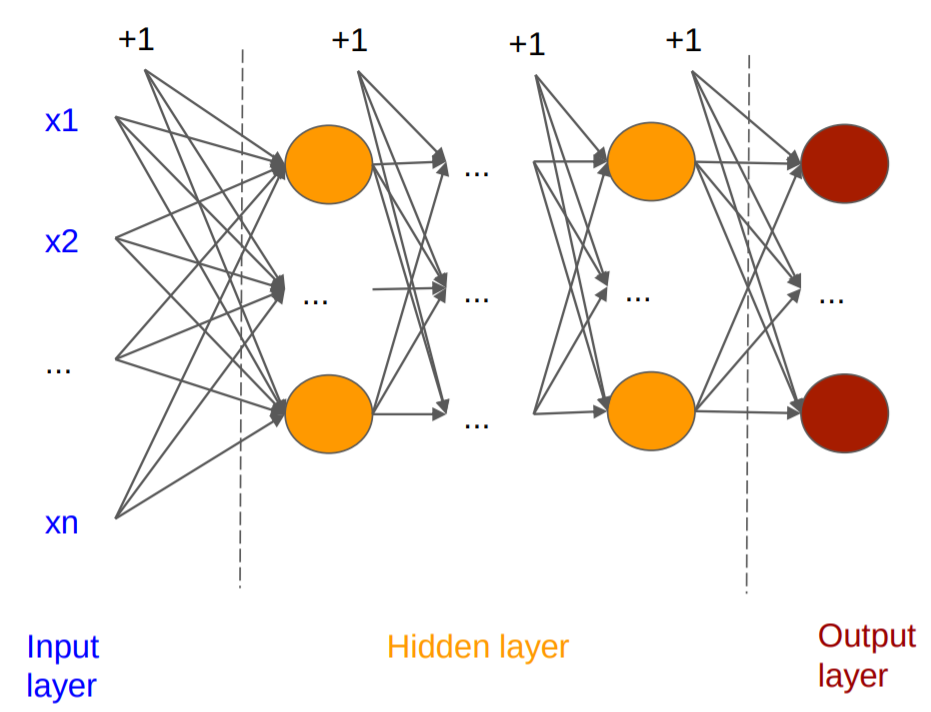
\includegraphics[width=0.4\textwidth]{resources/ilustrasi_ann.png}
	    }
	    \caption{Ilustrasi ANN \cite{b6}.}
	    \label{fig:ilustrasi_ann}
	\end{figure}

	Pada fase \textit{forward propagation}, tiap input numerik diproses sesuai dengan bobot dari tiap neuronnya. Output suatu neuron akan menjadi input dari neuron pada lapisan setelahnya. Pada Gambar \ref{fig:ilustrasi_neuron}, diberikan input numerik riil berupa \(X_1, X_2, \ldots, X_n\) (\(X_0 = 1\) sebagai bias), bobot \(W_0, W_1, W_2, \ldots, W_n\), dan sebuah fungsi aktifasi \(f\). Maka output dikomputasi dengan hitungan pada \ref{eq:1_ann}.

	\begin{equation}
		output = f(\sum_{i=0}^{n}x_iw_i)
		\label{eq:1_ann}
	\end{equation} 

	\begin{figure}[htbp]
	    \centerline{
	    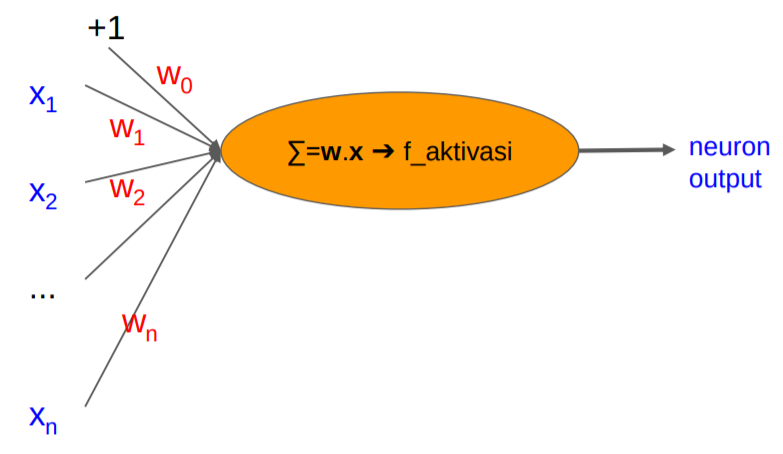
\includegraphics[width=0.4\textwidth]{resources/ilustrasi_neuron.png}
	    }
	    \caption{Ilustrasi suatu neuron \cite{b6}.}
	    \label{fig:ilustrasi_neuron}
	\end{figure}

	Komputasi output dilakukan hingga lapisan terakhir. Setelah output didapatkan, maka pembelajaran masuk fase \textit{backpropagation}. Pada fase ini kesalahan antara output prediksi dihitung dengan output seharusnya dan diteruskan kebelakang. Melalui error yang sudah dikomputasi ini kemudia bobot diperbaharui pada fase terakhir. Dengan melakukan proses ini terus menerus hingga diperoleh \textit{error} yang minimum, dapat diperoleh algoritme yang mangkus mengaproksimasi fungsi aslinya.

	\subsection{Penggunaan ANN di Word2Vec dan Representasi Teks Lintas Bahasa}
	Salah satu bentuk dari Transfer Learning adalah pembelajaran lintas bahasa \cite{b7}. Pada pembelajaran lintas bahasa, pembelajaran pertama-tama dilakukan di bahasa lain yang lebih populer dan kemudian digunakan pada bahasa lain yang lebih tidak populer. Untuk dapat melakukan hal ini, diperlukan representasi bahasa pada ruang yang sama seperti dapat dilihat pada ilustrasi di gambar \ref{fig:ilustrasi_embedding}.

	\begin{figure}[htbp]
	    \centerline{
	    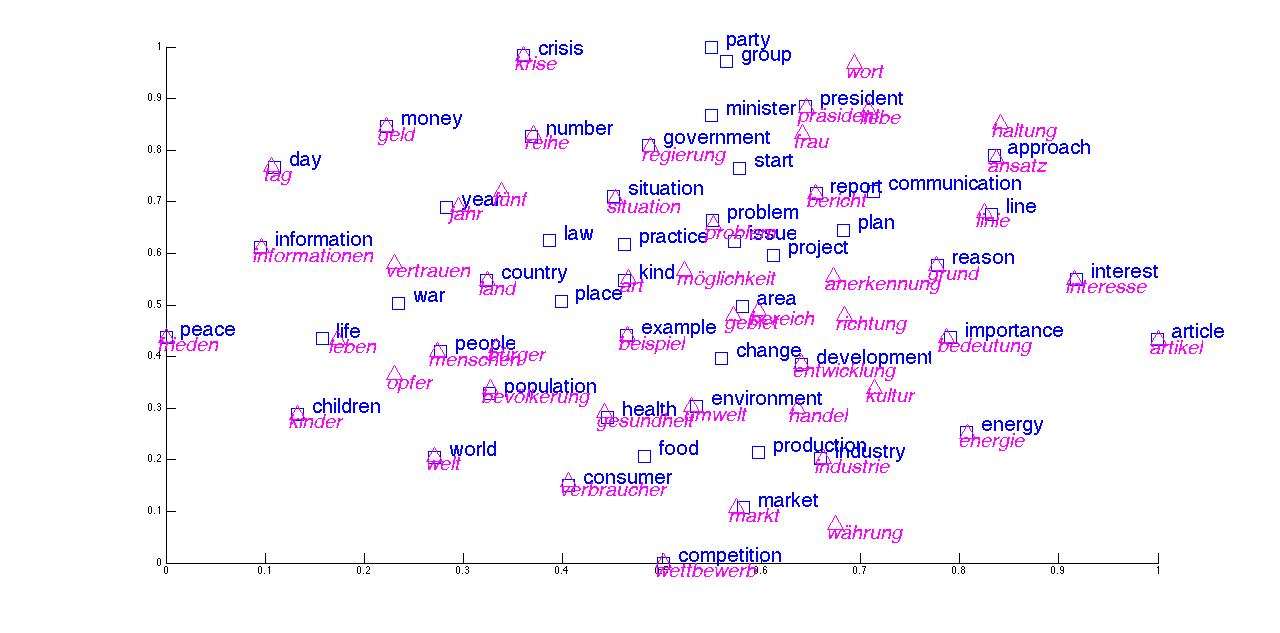
\includegraphics[width=0.5\textwidth]{resources/luong_et_al_2015.jpg}}
	    \caption{Ilustrasi ruang \textit{embedding} antara dua bahasa \cite{b8}.}
	    \label{fig:ilustrasi_embedding}
	\end{figure}

	Sebelumnya, diperlukan ahli untuk membangun kamus kata-kata dan kalimat secara manual untuk dapat membandingkan kata dari dua bahsa. Seiring dengan perkembangan teknologi, berbagai teknik berkembang untuk dapat melakukan hal ini secara otomatis. Berdasarkan \cite{b9}, secara garis besar terdapat 2 pendekatan berbeda dalam membangun ruang \textit{embedding} antar bahasa:

	\begin{enumerate}
	    \item \textit{Monolingual mapping}: Pada teknik ini, model dilatih secara independen pada bahasa masing-masing. Kemudian mapping antara bahasa dipelajari untuk mendapatkan representasi antar bahasa.

	    \item \textit{Joint optimization}: Pada teknik ini, model dilatih pada korpus antar bahasa. Model kemudian mengoptimisasi kombinasi dari monolingual dan cross-lingual loss.
	\end{enumerate}

	Pada \textit{monolingual mapping}, salah satu teknik adalah dengan pertama-tama mempelajari representasi bahasa menggunakan model Skip-gram atau Continuous Bag-of-Words (CBOW) yang didistribusikan diusulkan oleh \cite{b10}. Model-model ini mempelajari representasi kata menggunakan arsitektur \textit{neural network} sederhana yang bertujuan untuk memprediksi tetangga kata. Karena kesederhanaannya, model Skip-gram dan CBOW dapat dilatih pada sejumlah besar data teks. Pada implementasi paralelnya model ini dapat belajar dari miliaran kata dalam hitungan jam.

	Baru-baru ini ditunjukkan bahwa representasi kata yang didistribusikan secara mengejutkan menangkap banyak keteraturan linguistik, dan ada banyak jenis kesamaan di antara kata-kata yang dapat dinyatakan sebagai terjemahan linear \cite{b11}. Misalnya, operasi vektor "raja" - "pria" + "wanita" menghasilkan vektor yang dekat dengan "ratu".

	Dua model khusus untuk mempelajari representasi kata yang dapat dilatih secara efisien pada banyak data teks adalah model Skip-gram dan CBOW yang diperkenalkan di \cite{b10}. Dalam model CBOW, tujuan pelatihannya adalah untuk menggabungkan representasi kata di sekitarnya untuk memprediksi kata di tengah. Sedangkan dalam model Skip-gram, tujuan pelatihan adalah untuk mempelajari representasi kata vektor yang pandai memprediksi konteksnya dalam kalimat yang sama \cite{b10}. Model arsitektur dari dua metode ini ditunjukkan pada Gambar \ref{fig:ilustrasi_cbow_skip_gram}.

	\begin{figure}[htbp]
	    \centerline{
	    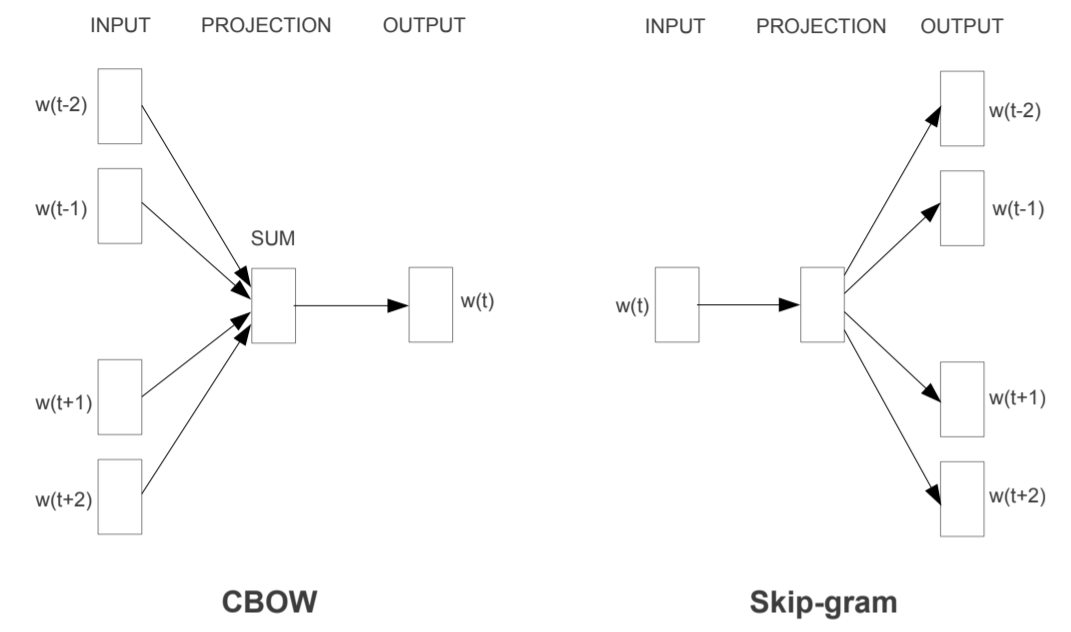
\includegraphics[width=0.5\textwidth]{resources/cbow-skip-gram-illustration.png}}
	    \caption[Ilustrasi model CBOW dan Skip-gram.]{ Dalam model CBOW, representasi konteks terdistribusi (atau kata-kata sekitarnya) digabungkan untuk memprediksi kata di tengah. Dalam model Skip-gram, representasi terdistribusi dari kata input digunakan untuk memprediksi kata-kata sekitarnya \cite{b12}.}
	    \label{fig:ilustrasi_cbow_skip_gram}
	\end{figure}

	Lebih formal, diberi urutan kata pelatihan \(w1, w2, w3,. . . , wT,\) tujuan dari model Skip-gram adalah untuk memaksimalkan probabilitas log rata-rata

	\begin{equation}
	    \frac{1}{T}\sum_{t=1}^{T}\begin{bmatrix}
	    \sum_{j=-k}^{K}{\log p(w_{t+j}|w_{t})}
	    \end{bmatrix}
	    \label{eq:1}
	\end{equation}

	di mana \(k\) adalah ukuran jendela pelatihan. Iterasi penjumlahan di bagian dalam berjalan dari \({-k}\) ke \(k\) untuk menghitung probabilitas log benarnya memprediksi kata \(w_{t+j}\) jika kata di tengah \(w_{t}\). Iterasi penjumlahan di luar mencakup semua kata dalam korpus pelatihan. 

	Ketika dilatih tentang dataset besar, model Skip-gram atau CBOW ini menangkap banyak informasi semantik. Seperti yang disebutkan sebelumnya, kata-kata yang berkaitan erat memiliki representasi vektor yang serupa, misalnya, sekolah dan universitas, danau, dan sungai. Ini karena sekolah dan universitas muncul dalam konteks yang sama, sehingga selama pelatihan representasi vektor dari kata-kata ini didorong untuk menjadi dekat satu sama lain. Lebih menarik lagi, vektor menangkap hubungan antara konsep melalui operasi linier. Misalnya, \(vektor(Prancis) - vektor(Paris)\) mirip dengan \(vektor(Italia) - vektor(Roma)\).

	Pada gambar \ref{fig:ilustrasi_embedding_inggris_spanyol}, dapat dilihat visualisasi hasil pembelajaran Skip-gram atau CBOW. Gambar \ref{fig:ilustrasi_embedding_inggris_spanyol} memvisualisasikan vektor untuk angka dan hewan dalam bahasa Inggris dan Spanyol, dan dapat dengan mudah dilihat bahwa konsep-konsep ini memiliki susunan geometris yang serupa. Hal ini dikarenakan semua bahasa umum memiliki konsep yang didasarkan pada dunia nyata (seperti kucing adalah binatang yang lebih kecil dari seekor anjing), sering kali ada kesamaan kuat antara ruang vektor. Kesamaan pengaturan geometris dalam ruang vektor adalah alasan utama mengapa metode ini dapat bekerja dengan baik.

	\begin{figure}[htbp]
	    \centerline{
	    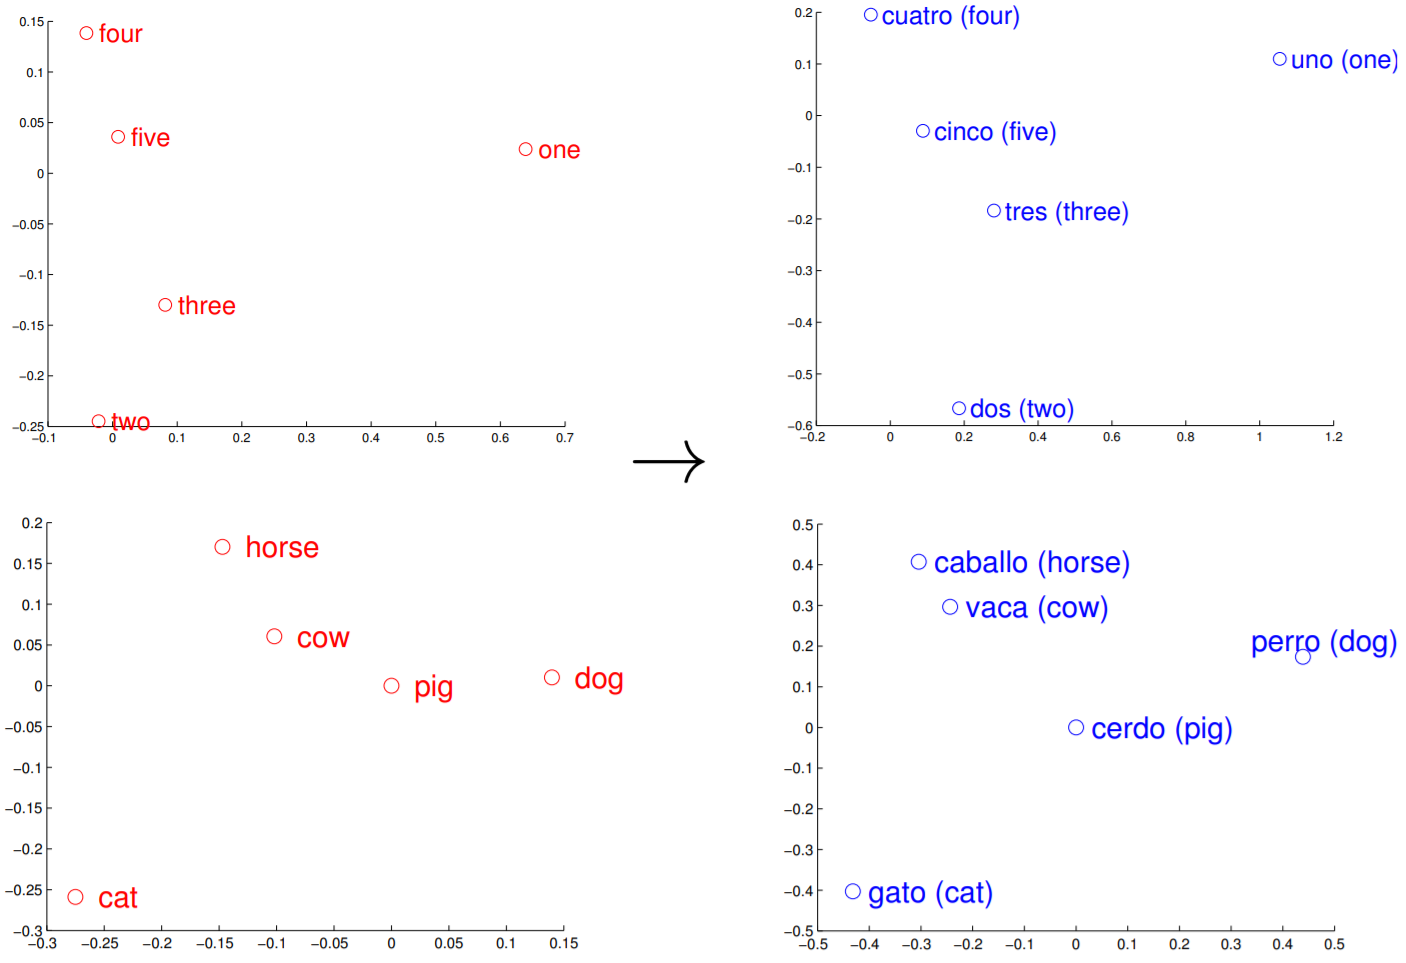
\includegraphics[width=0.5\textwidth]{resources/ilustration-eng-spn-word.png}}
	    \caption[Ilustrasi ruang \textit{embedding} antara bahasa Inggris dan Spanyol \cite{b12}.]{ Vektor yang sudah dipelajari diproyeksikan ke ruang dua dimensi menggunakan PCA dan dirotasi.}
	    \label{fig:ilustrasi_embedding_inggris_spanyol}
	\end{figure}

	Dikarenakan miripnya representasi bahasa, jika kita mengetahui translasi beberapa objek, contoh angka satu sampai lima, kita dapat menyesuaikan representasi antar bahasa dengan rotasi, \textit{scaling}, dan translasi untuk mendapatkan tranlasi angka lainnya. Lebih formalnya, misalkan diberi satu set pasangan kata dan representasi vektor yang terkait \begin{math} \begin{Bmatrix} {x_{i}, z_{i}} \end{Bmatrix}_{i=1}^{n} \end{math}, di mana \(x_{i}\in\mathbb{R}^{d_{1}}\) adalah representasi terdistribusi dari kata i dalam bahasa sumber, dan \(z_{i}\in\mathbb{R}^{d_{2}}\) adalah representasi vektor dari terjemahannya. Kemudian dicari matriks transformasi \( W\) sehingga \(W x_{i}\) mendekati \(z_{i}\). Dalam praktiknya, \(W\) dapat dipelajari dengan masalah optimasi berikut

	\begin{equation}
	    \min_{W}\sum_{i=1}^{n}\left \| Wx_i-z_i \right \|^2
	    \label{eq:2}
	\end{equation}

	yang dapat diselesaikan dengan \textit{stochastic gradient descent} \cite{b12}.

	Pada saat melakukan prediksi, untuk setiap kata baru yang diberikan dan representasi vektor kontinu \(x\), kita dapat memetakannya ke ruang bahasa lain dengan menghitung \(z = W x\). Kemudian kita dapat menemukan kata yang representasinya paling dekat dengan \(z\) dalam ruang bahasa target, menggunakan \textit{cosine similarity} sebagai metrik jarak. Terlepas dari kesederhanaannya, metode transformasi linier ini bekerja dengan baik dalam eksperimen yang \cite{b12} jalankan, lebih baik daripada teknik \textit{nearest neighbour} dan juga pengklasifikasi \textit{neural network}.

	Meski \textit{monolingual mapping} sukses mendapatkan ruang \textit{embedding} antar bahasa, teknik ini mahal dan susah diaplikasikan ke bahasa yang memiliki sumber daya rendah. Untuk dapat mengaplikasikan teknik ini diperlukan kamus kata-kata atau kalimat paralel antar bahasa, hal yang seringkali tidak tersedia pada bahasa bersumber daya rendah. Oleh karena itu, mengaplikasikan teknik ini sangat sulit pada bahasa Indonesia. 

\begin{figure*}[htb]
    \centerline{
    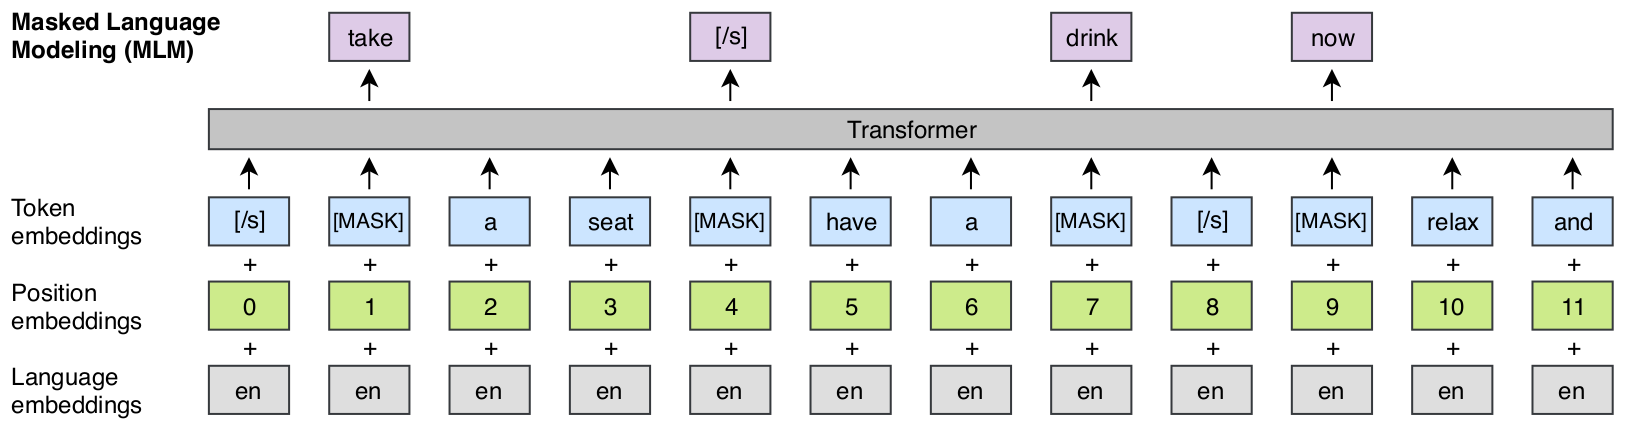
\includegraphics[width=1\textwidth]{resources/ilustrasi-mlm.png}}
    \caption{Ilustrasi \textit{masked language modeling} \cite{b2}.}
    \label{fig:ilustrasi_mlm}
\end{figure*}

\section{Transformer}
Teknik pembelajaran \textit{Transformer}, yang termasuk jenis \textbf{\textit{discriminative}}, pertama kali dimodelkan pada tahun 2017 oleh Vaswani dkk. \cite{b14}. Perkembangan topologi ini berhasil mendorong performa pada berbagai dataset tolak ukur seperti GLUE \cite{b15}. Sub-bab selanjutnya akan menjelaskan lebih detil mengenai teknik dan penggunaannya.

	\subsection{Teknik Pembelajaran}
	Berdasarkan \cite{b14}, arsitektur \textit{Transformer} terdiri dari \textit{self-attention} dan \textit{point-wise} yang ditumpuk, dan \textit{fully connected layer} untuk enkoder dan dekoder. Ilustrasi secara keseluruhan arsitektur \textit{Transformer} dapat dilihat pada Gambar \ref{fig:ilustrasi_transformer}.

	\begin{figure}[htbp]
	    \centerline{
	    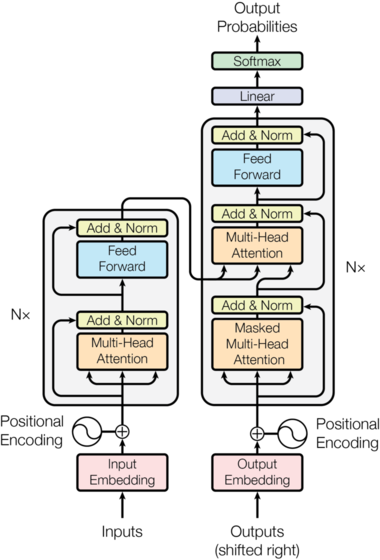
\includegraphics[width=0.2\textwidth]{resources/overview-transformer.png}}
	    \caption{Ilustrasi \textit{transformer} secara keseluruhan \cite{b14}.}
	    \label{fig:ilustrasi_transformer}
	\end{figure}

	Fungsi \textit{attention} dapat digambarkan sebagai memetakan kueri dan pasangan \textit{key-value} untuk suatu output, di mana kueri (Q), kunci (K), nilai (V), dan \textit{output} semuanya vektor. \textit{Output} dihitung sebagai \textit{weighted sum} dari nilai-nilai, di mana bobot yang ditetapkan untuk setiap nilai dihitung oleh fungsi kompatibilitas kueri dari kunci yang sesuai.

	Pada penelitian \cite{b14}, tipe \textit{attention} ini disebut "\textit{Scaled Dot-Product Attention}". Input terdiri dari kueri dan kunci dimensi \(d_{k}\), dan nilai dimensi \(d_{v}\). \textit{Dot product} dari kueri dihitung dengan semua kunci, membaginya dengan \(\sqrt{d_{k}}\), dan menerapkan fungsi softmax untuk mendapatkan bobot pada nilai. Ilustrasi \textit{attention} dapat dilihat pada Gambar \ref{fig:ilustrasi_attention}.

	\begin{figure}[htbp]
	    \centerline{
	    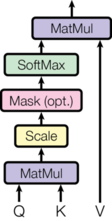
\includegraphics[width=0.1\textwidth]{resources/overview-attention.png}}
	    \caption{Ilustrasi \textit{attention} secara keseluruhan \cite{b14}.}
	    \label{fig:ilustrasi_attention}
	\end{figure}

	Pada prakteknya, hasil keluaran fungsi \textit{attention} pada sebuah set kueri dihitung secara besamaan, dikemas bersama menjadi matriks Q. Kunci dan nilai juga dikemas bersama menjadi matriks K dna V. Kemudian hasil keluaran dapat dihitung dengan:

	\begin{equation}
	    Attention(Q,K,V) = softmax(\frac{QK^{T}}{\sqrt{d_k}})V
	\end{equation}

	Dengan menggunakan arsitektur ini, didapatkan kemajuan terbaru dalam representasi teks dengan teknik \textit{joint optimization}. Teknik \textit{joint optimization} yang sebelumnya memerlukan korpus paralel atau kamus bilingual (\textit{supervised}) \cite{b13}, kini dapat dilakukan tanpa korpus paralel atau kamus bilingual (\textit{unsupervised}) \cite{b2}. Hal ini dilakukan dengan memanfaatkan \textit{shared sub-word vocabulary}. Tidak hanya itu, \cite{b2} juga memanfaatkan \textit{masked language modeling} dan arsitektur \textit{transformer} untuk mendapatkan \textit{language model} yang mangkus. Sub-bab selanjutnya akan membahas detail \textit{shared sub-word vocabulary} dan \textit{masked language modeling} dari \textit{language model pretraining} lintas bahasa bernama XLM yang dikembangkan oleh \cite{b2}.

\begin{figure*}[!htb]
    \centerline{
    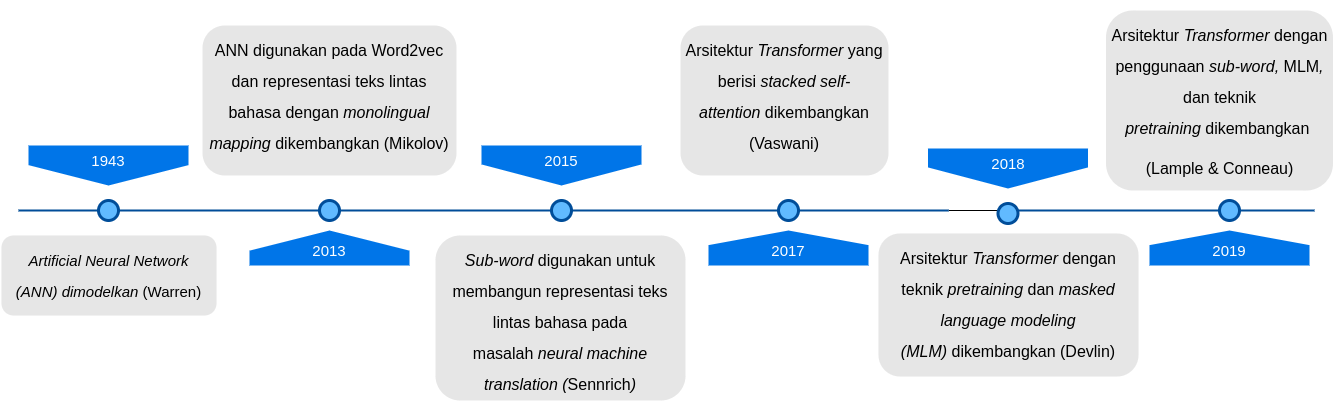
\includegraphics[width=1\textwidth]{resources/timeline.png}}
    \caption{Timeline perkembangan}
    \label{fig:timeline}
\end{figure*}

	\subsection{Shared sub-word vocabulary}
	Berdasarkan penelitian oleh \cite{b16}, salah satu inspirasi menggunakan \textit{sub-word} adalah fakta bahwa terjemahan beberapa kata bersifat transparan karena terjemahannya dapat diterjemahkan oleh penerjemah yang kompeten, bahkan jika itu adalah kata yang belum pernah ditemui, berdasarkan terjemahan dari \textit{sub-word} yang dikenal seperti morfemnya atau fonemnya. Kategori kata yang terjemahannya berpotensi transparan meliputi:

	\begin{enumerate}
	    \item Entitas bernama (\textit{named entities}). Di antara bahasa yang menggunakan alfabet, nama seringkali dapat disalin dari sumber ke teks target. Transkripsi atau transliterasi mungkin diperlukan pada bahasa dengan huruf atau suku kata berbeda. Contoh: \\
	    Barack Obama (Bahasa Inggris dan Jerman) \\
	    \foreignlanguage{russian}{Барак Обама} (Bahasa Rusia) \\
	    \begin{CJK}{UTF8}{min}
	    バラク・オバマ (ba-ra-ku o-ba-ma) (Bahasa Jepang)
	    \end{CJK}

	    \item Kata-kata serumpun dan pinjaman. Kata serumpun dan kata pinjaman dengan asal yang sama dapat berbeda secara reguler antar bahasa, sehingga aturan penerjemahan tingkat karakter sudah cukup \cite{b17}. Contoh:  \\
	    claustrophobia (Bahasa Inggris) \\
	    Klaustrophobie (Bahasa Jerman) \\
	    \foreignlanguage{russian}{Клаустрофобия} (Klaustrofobiâ) (Bahasa Rusia)

	    \item Kata-kata yang rumit secara morfologis. Kata-kata yang mengandung banyak morfem, misalnya yang dibentuk melalui peracikan, afiksasi, atau infleksi, dapat diterjemahkan dengan menerjemahkan morfem secara terpisah. Contoh:  \\
	    solar system (Bahasa Inggris) \\
	    Sonnensystem (Sonne + System) (Bahasa Jerman) \\
	    Naprendszer (Nap + Rendszer) (Bahasa Hongaria)
	\end{enumerate}

	Penelitian \cite{b16} membuktikan bahwa segmentasi kata-kata langka ke dalam unit \textit{sub-word} yang sesuai sudah cukup untuk memungkinkan \textit{neural translation network} mempelajari terjemahan yang transparan, dan menggeneralisasikan pengetahuan ini untuk menerjemahkan dan menghasilkan kata-kata yang tidak ditemui sebelumnya. Pada penelitiannya, mereka menggunakan teknik \textit{Byte Pair Encoding} untuk mendapatkan tidak hanya \textit{sub-word}-nya tetapi juga kompresi dari kamus-kamus kata yang ada.

	Teknik \textit{Byte Pair Encoding} (BPE) \cite{b18} adalah teknik kompresi data sederhana yang secara iteratif menggantikan pasangan \textit{byte} yang paling sering muncu; secara berurutan dengan \textit{byte} tunggal yang tidak digunakan. Pada penelitiannya, \cite{b16} mengadaptasi algoritma \textit{Byte Pair Encoding} untuk segmentasi kata. Alih-alih sering menggabungkan pasangan \textit{byte}, mereka menggabungkan karakter atau urutan karakter.

	Pertama-tama, kosakata simbol diinisialisasi dengan kosakata karakter, dan mewakili setiap kata sebagai urutan karakter, ditambah simbol akhir kata khusus ‘·’, yang memungkinkan hasil terjemahan dikembalikan ke bentuk awal setelah terjemahan. Kemudian semua pasangan simbol dihitung secara iteratif dan untuk setiap pasangan yang paling sering diganti dengan simbol baru. Contoh ('A', 'B') menjadi 'AB'. Setiap operasi penggabungan menghasilkan simbol baru yang mewakili \textit{n-gram} dari karakter. Karakter yang sering muncul (atau seluruh kata) pada akhirnya digabungkan menjadi satu simbol. Ukuran kosa kata simbol akhir sama dengan ukuran kosa kata awal, ditambah jumlah operasi penggabungan --- yang merupakan satu-satunya \textit{hyperparameter} dari algoritma.

	Dapat dilihat contoh sederhana algoritma \textit{Byte Pair Encoding} pada Lampiran \ref{appendix:simple_bpe_algorithm} oleh \cite{b16}. Pada algoritma ini, operasi \textit{Byte Pair Encoding} belajar dari kamus kata {‘low’, ‘lower’, ‘newest’, ‘widest’}. Pada akhir iterasi, akan diperoleh representasi dari kamus kata dalam bentuk simbol-simbol yang dipelajari. Pada contoh tersebut, kata 'lowest' yang berada diluar kamus kata akan direpresentasikan menjadi gabungan dari simbol 'low' dan 'est'. Di sini dapat dilihat bagaimana \textit{Byte Pair Encoding} dapat membantu merepresentasikan kata yang berada diluar kamus kata. 

	\subsection{Masked Language Modeling (MLM)}
	Dideskripsikan pada penelitian oleh \cite{b19}, \textit{Masked Language Modeling} terinspirasi dari \textit{Cloze task} \cite{b20}. Teknik MLM secara acak akan menyembunyikan beberapa kata dari input, dan model memiliki objektif untuk menebak kata asli dari kata yang disembunyikan tadi berdasarkan konteks yang ada di sekelilingnya. Tidak seperti pelatihan \textit{language model} lainnya yang berjalan dari kiri-ke-kanan, pelatihan dengan objektif MLM memungkinkan representasi dari kiri dan kanan mengambil peran. Hal ini memungkinkan kita untuk melatih \textit{Transformer} secara dua arah. Ilustrasi dari \textit{masked language modeling} secara keseluruhan dapat dilihat pada Gambar \ref{fig:ilustrasi_mlm}.
	
	Sama dengan BERT \cite{b19}, persentase dari kata yang akan dipilih untuk disembunyikan pada XLM adalah 15 persen. Setelah sebuah posisi dipilih secara acak, sebuah kata kemudian memiliki 80 persen kemungkinan untuk disembunyikan, 10 persen kemungkinan untuk diganti menjadi sebuah kata acak, dan 10 persen kemungkinan tidak diganti sama sekali.

\section{Analisis dan Kesimpulan}
Teknik representasi teks lintas bahasa telah berkembang jauh seperti yang dapat dilihat pada Gambar \ref{fig:timeline}. Pada awalnya, representasi teks lintas bahasa harus didapatkan melalui melatih ANN dengan teknik CBOW atau Skip-gram. Setelah didapatkan representasi tiap bahasa, dilakukan \textit{monolingual mapping} dengan menggunakan korpus paralel atau kamus bilingual untuk mendapatkan representasi teks lintas bahasa. Teknik ini sangat mahal untuk dilakukan dikarenakan jarang tersedia korpus paralel atau kamus bilingual untuk bahasa seperti bahasa Indonesia. Selain itu, teknik ini juga tidak mangkus dalam prakteknya dikarenakan dangkalnya model yang digunakan.

Perkembangan terbaru dengan memanfaatkan \textit{shared sub-word vocabulary}, arsitektur \textit{transformer}, dan teknik \textit{masked language modeling} berhasil mempermudah dan meningkatkan efektivitas teknik sebelumnya. Dengan menggunakan \textit{shared sub-word vocabulary}, representasi teks lintas bahasa bisa didapatkan tanpa memerlukan korpus paralel atau kamus bilingual. Selain itu, dengan menggunakan arsitektur \textit{transformer} dan teknik \textit{masked language modeling}, model dapat lebih mangkus mempelajari representasi teks lintas bahasa. Hal ini dibuktikan dengan memperoleh hasil tertinggi dalam dataset tolak ukur lintas bahasa XNLI \cite{b21}.

\begin{thebibliography}{00}
\bibitem{b1} Tomas Mikolov et al. “Distributed Representations of Words and Phrases andtheir Compositionality”. In: arXiv:1310.4546 [cs, stat] (2013). arXiv: 1310.4546.URL :http://arxiv.org/abs/1310.4546.
\bibitem{b2} Guillaume Lample \& Alexis Conneau. “Cross-lingual Language Model Pre-training”. In: arXiv:1901.07291 [cs] (2019). arXiv: 1901.07291.
URL :http://arxiv.org/abs/1901.07291.
\bibitem{b3} McCulloch, Warren; Walter Pitts. (1943). "A Logical Calculus of Ideas Immanent in Nervous Activity". Bulletin of Mathematical Biophysics. 5 (4): 115–133. doi:10.1007/BF02478259
\bibitem{b4} Ng, Andrew; Dean, Jeff. (2012). "Building High-level Features Using Large Scale Unsupervised Learning". arXiv:1112.6209
\bibitem{b5} A. Krizhevsky, I. Sutskever, and G. Hinton. Imagenet classification with deep convolutional neural networks. In NIPS, 2012.
\bibitem{b6} Masayu Leylia Khodra \& Dessi Puji Lestari. (2019). "Regresi dan ANN". URL: http://stei.kuliah.itb.ac.id
\bibitem{b7} Sebastian Ruder et al. “Transfer Learning in Natural Language Processing”. In: Proceedings of the 2019 Conference of the North American Chapter of the As- sociation for Computational Linguistics: Tutorials. 2019, pp. 15–18.
\bibitem{b8} Thang Luong, Hieu Pham \& Christopher D. Manning. “Bilingual Word Repre- sentations with Monolingual Quality in Mind”. In: Proceedings of the 1st Work- shop on Vector Space Modeling for Natural Language Processing. Association for Computational Linguistics, 2015, 151–159. URL : https://www.aclweb.org/anthology/W15-1521. DOI :10.3115/v1/W15-1521.
\bibitem{b9} Zirui Wang et al. “Cross-lingual Alignment vs Joint Training: A Comparative Study and A Simple Unified Framework”. In: arXiv:1910.04708 [cs] (2019). arXiv: 1910.04708. URL : http://arxiv.org/abs/1910.04708.
\bibitem{b10} Tomas Mikolov et al. “Efficient Estimation of Word Representations in Vector Space”. In: arXiv:1301.3781 [cs] (2013). arXiv: 1301.3781. URL : https://arxiv.org/abs/1301.3781.
\bibitem{b11} Tomas Mikolov, Wen-tau Yih \& Geoffrey Zweig. “Linguistic Regularities in Continuous Space Word Representations”. In: Proceedings of the 2013 Con- ference of the North American Chapter of the Association for Computational Linguistics: Human Language Technologies. Association for Computational Linguistics, 2013, 746–751. URL : https://www.aclweb.org/anthology/N13-1090.
\bibitem{b12} Tomas Mikolov, Quoc V. Le \& Ilya Sutskever. “Exploiting Similarities among Languages for Machine Translation”. In: arXiv:1309.4168 [cs] (2013). arXiv: 1309.4168. URL : http://arxiv.org/abs/1309.4168.
\bibitem{b13} Chao Xing et al. “Normalized Word Embedding and Orthogonal Transform for Bilingual Word Translation”. In: Proceedings of the 2015 Conference of the Nor- th American Chapter of the Association for Computational Linguistics: Human Language Technologies. 2015.
\bibitem{b14} Ashish Vaswani et al. “Attention Is All You Need”. In: arXiv:1706.03762 [cs] (2017). arXiv: 1706.03762. URL : http://arxiv.org/abs/1706.03762.
\bibitem{b15} Alex Wang et al. “GLUE: A Multi-Task Benchmark and Analysis Platform for Natural Language Understanding”. In: arXiv:1804.07461 [cs] (2019). arXiv: 1804.07461. URL : http://arxiv.org/abs/1804.07461.
\bibitem{b16} Rico Sennrich, Barry Haddow \& Alexandra Birch. “Neural Machine Translation of Rare Words with Subword Units”. In: arXiv:1508.07909 [cs] (2016). arXiv: 1508.07909. URL : http://arxiv.org/abs/1508.07909.
\bibitem{b17} Jörg Tiedemann. “Character-Based Pivot Translation for Under-Resourced Languages and Domains”. In: Proceedings of the 13th Conference of the European Chapter of the Association for Computational Linguistics. Association for Computational Linguistics, 2012, 141–151. URL : https://www.aclweb.org/anthology/E12-1015.
\bibitem{b18} Philip Gage. “A New Algorithm for Data Compression”. In: C Users J. 12.2 (1994), 23–38. ISSN : 0898-9788.
\bibitem{b19} Jacob Devlin et al. “BERT: Pre-training of Deep Bidirectional Transformers for Language Understanding”. In: arXiv:1810.04805 [cs] (2019). arXiv: 1810.04805. URL : http://arxiv.org/abs/1810.04805.
\bibitem{b20} Wilson L. Taylor. ““Cloze Procedure”: A New Tool for Measuring Readability”. In: Journalism Quarterly 30.4 (1953), 415–433. ISSN : 0022-5533. DOI :10.1177/107769905303000401.
\bibitem{b21} Alexis Conneau et al. “XNLI: Evaluating Cross-lingual Sentence Representations”. In: Proceedings of the 2018 Conference on Empirical Methods in Natural Language Processing. Association for Computational Linguistics, 2018, 2475–2485. DOI : 10.18653/v1/D18- 1269. URL :https://www.aclweb.org/anthology/D18-1269.
\end{thebibliography}

\clearpage
\appendices
	\section{Algoritma \textit{Byte Pair Encoding} Sederhana}
	\label{appendix:simple_bpe_algorithm}

	Algoritma (contoh nama file: \(bpe.py\)):
	\begin{lstlisting}[language=Python]
	import re, collections
	def get_stats(vocab):
	    pairs = collections.defaultdict(int)
	    for word, freq in vocab.items():
	        symbols = word.split()
	        for i in range(len(symbols)-1):
	            pairs[symbols[i],symbols[i+1]] += freq
	    return pairs

	def merge_vocab(pair, v_in):
	    v_out = {}
	    bigram = re.escape(' '.join(pair))
	    p = re.compile(r'(?<!\S)' + bigram + r'(?!\S)')
	    for word in v_in:
	        w_out = p.sub(''.join(pair), word)
	        v_out[w_out] = v_in[word]
	    return v_out

	vocab = {'l o w </w>' : 5, 'l o w e r </w>' : 2,
	'n e w e s t </w>':6, 'w i d e s t </w>':3}
	vocab_test = {'l o w e s t </w>': 1}

	num_merges = 10
	for i in range(num_merges):
	    pairs = get_stats(vocab)
	    best = max(pairs, key=pairs.get)
	    print('~~~')
	    vocab = merge_vocab(best, vocab)
	    vocab_test = merge_vocab(best, vocab_test)
	    print("best: ", best)
	    print("vocab: ", vocab)
	    print("vocab_test: ", vocab_test)
	\end{lstlisting}

	Setelah dijalankan di mesin bersistem operasi Ubuntu 18.04 dengan perintah
	\begin{lstlisting}[language=bash]
	    $ python3 bpe.py
	\end{lstlisting}

	akan didapatkan keluaran sebagai berikut:
	\begin{lstlisting}[language=bash]
	~~~
	best:  ('e', 's')
	vocab:  {'l o w </w>': 5, 'l o w e r </w>': 2, 'n e w es t </w>': 6, 'w i d es t </w>': 3}
	vocab_test:  {'l o w es t </w>': 1}
	~~~
	best:  ('es', 't')
	vocab:  {'l o w </w>': 5, 'l o w e r </w>': 2, 'n e w est </w>': 6, 'w i d est </w>': 3}
	vocab_test:  {'l o w est </w>': 1}
	~~~
	best:  ('est', '</w>')
	vocab:  {'l o w </w>': 5, 'l o w e r </w>': 2, 'n e w est</w>': 6, 'w i d est</w>': 3}
	vocab_test:  {'l o w est</w>': 1}
	~~~
	best:  ('l', 'o')
	vocab:  {'lo w </w>': 5, 'lo w e r </w>': 2, 'n e w est</w>': 6, 'w i d est</w>': 3}
	vocab_test:  {'lo w est</w>': 1}
	~~~
	best:  ('lo', 'w')
	vocab:  {'low </w>': 5, 'low e r </w>': 2, 'n e w est</w>': 6, 'w i d est</w>': 3}
	vocab_test:  {'low est</w>': 1}
	~~~
	best:  ('n', 'e')
	vocab:  {'low </w>': 5, 'low e r </w>': 2, 'ne w est</w>': 6, 'w i d est</w>': 3}
	vocab_test:  {'low est</w>': 1}
	~~~
	best:  ('ne', 'w')
	vocab:  {'low </w>': 5, 'low e r </w>': 2, 'new est</w>': 6, 'w i d est</w>': 3}
	vocab_test:  {'low est</w>': 1}
	~~~
	best:  ('new', 'est</w>')
	vocab:  {'low </w>': 5, 'low e r </w>': 2, 'newest</w>': 6, 'w i d est</w>': 3}
	vocab_test:  {'low est</w>': 1}
	~~~
	best:  ('low', '</w>')
	vocab:  {'low</w>': 5, 'low e r </w>': 2, 'newest</w>': 6, 'w i d est</w>': 3}
	vocab_test:  {'low est</w>': 1}
	~~~
	best:  ('w', 'i')
	vocab:  {'low</w>': 5, 'low e r </w>': 2, 'newest</w>': 6, 'wi d est</w>': 3}
	vocab_test:  {'low est</w>': 1}
	\end{lstlisting}

\end{document}
